\section{Technische Konzepte}\label{technische_konzepte}
Im vorherigen Kapitel wurden viele Aufgaben aufgedeckt, die im Kontext eines Software Shops entstehen. Einige dieser Aufgaben, wie die Sicherheitsverifikation und die Klassifizierung von Software benötigen zur möglichen Bearbeitung Konzepte zur Bewertung. Hierzu wird zunächst ein mögliches Klassifikationskonzept für Software vorgestellt. In diesem werden Berechtigungen und Kennzahlen von Softwares vorgestellt. Durch das Klassifizieren von Software können bei der Suche nach Software bereitgestellte Filter genutzt werden, welche Kunden bei der Suche der gewünschten Software unterstützt. Im Anschluss daran werden in Kapitel \ref{4.2} drei Kommunikationskonzepte vorgestellt, welche den Ablauf der Kommunikation zwischen Fahrzeug, Server und anderen Akteuren der Umwelt im Kontext bestimmter Anwendungsfälle darstellen.

\subsection{Klassifizierung von Software}\label{sw_klassifizierung}
Das Ziel der Software Klassifikation ist es, dem Kunden beim Kauf unterstützende Kennzahlen und Gruppierungen zur Verfügung zu stellen. Anhand dieser können sinnvollere Kaufentscheidungen getätigt werden und Kunden erhalten potentiell einen größeren Wert von der gekauften Software, wodurch die Wahrscheinlichkeit eines weiteren Kaufs steigen kann.\footnote{quelle}

\subsubsection{Berechtigungen und Details}
Eine dieser Kennzahlen ist die Anzahl genutzter Berechtigungen des Fahrzeugs. Nicht nur die Anzahl, sondern auch der Umfang einer Berechtigung können Kunden vom Kauf abschrecken.\footnote{quelle: android buch(1)} Eine Berechtigung muss der Software vom Fahrer erteilt worden sein, um die entsprechenden Dienste ausführen zu können. Eine Berechtigung erteilt der Software den Zugriff auf mögliche Systeme des Fahrzeugs. Einige Softwares können daher nicht genutzt werden, wenn ihnen nicht alle benötigten Berechtigungen erteilt wurden. Im Kontext intelligenter Fahrzeuge können mögliche Berechtigungen von der Architektur dieser abgeleitet werden, welche in Abbildung \hyperref[img:av_architecture]{9} dargestellt wird. Berechtigungen werden von den Entwicklern zur Software hinzugefügt und sind somit direkt zum auslesen im Shop verfügbar.

\begin{figure}[!h]
	\centering
	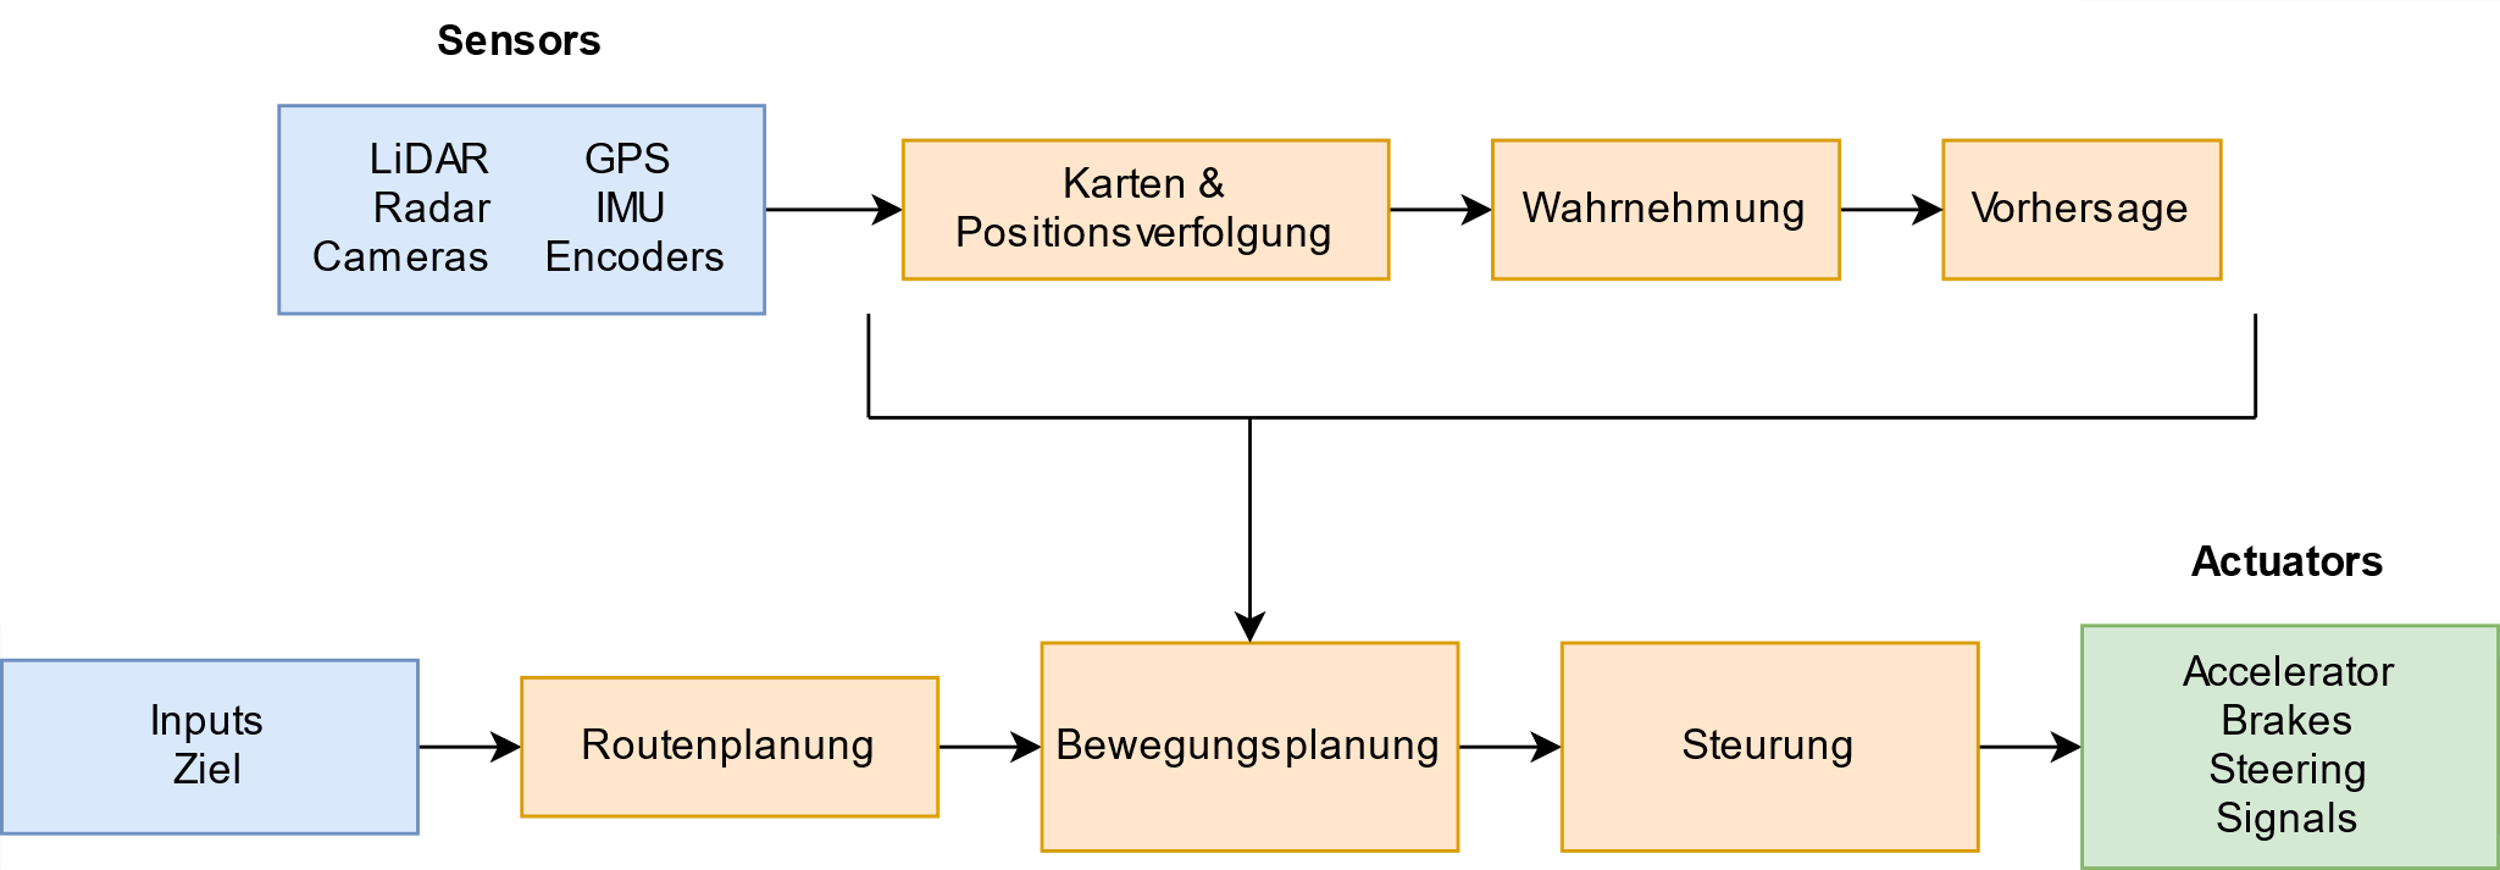
\includegraphics[width=\columnwidth]{pictures/arichtecture_AV.png}
	\label{img:av_architecture}
	\caption{Jeff Schneider: Architecture of Autonomous Vehicles}
\end{figure}

Berechtigungen können in zwei Gruppen unterteilt werden. \textit{"Normale"} Berechtigungen benötigen keiner direkten Zustimmung der Fahrzeughalter, da ihre alleinige Nutzung ungefährlich ist. \textit{"Kritische"} Berechtigungen sind solche, die im direkten Bezug zur Privatsphäre des Fahrzeughalters stehen. Für diese müssen Fahrzeughalter den Berechtigungen direkt zustimmen. Jede Berechtigung erlaubt es der Software bestimmte weitere Daten des Fahrzeugs zu lesen oder zu beeinflussen.\\\\
\large\textbf{Normale Berechtigungen}
\normalsize
\begin{itemize}
	\item[]\hspace{-0.6cm} \textbf{READ\_PERCEPTION}
	\item[]\hspace{-0.6cm} \textbf{READ\_PREDICTIONS}
	\item[]\hspace{-0.6cm} \textbf{READ\_CONTROLS}
	\item[]\hspace{-0.6cm} \textbf{READ\_ACTUATOR\_X}
\end{itemize}
\large\textbf{Kritische Berechtigungen}
\normalsize
\begin{itemize}
	\item[]\hspace{-0.6cm} \textbf{READ\_SENSOR\_X}
	\item[]\hspace{-0.6cm} \textbf{READ\_TRACKING}
	\item[]\hspace{-0.6cm} \textbf{READ\_ROUTE\_PLANNING}
	\item[]\hspace{-0.6cm} \textbf{READ\_MOVEMENT\_PLANNING}
	\item[]\hspace{-0.6cm} \textbf{READ\_KAMERA\_X}
	\item[]\hspace{-0.6cm} \textbf{INPUT\_NEW\_GOAL}
	\item[]\hspace{-0.6cm} \textbf{FEED\_TRACKING}
	\item[]\hspace{-0.6cm} \textbf{FEED\_PERCEPTION}
	\item[]\hspace{-0.6cm} \textbf{FEED\_PREDICTIONS}
	\item[]\hspace{-0.6cm} \textbf{FEED\_ROUTE\_PLANNING}
	\item[]\hspace{-0.6cm} \textbf{FEED\_MOVEMENT\_PLANNING}
	\item[]\hspace{-0.6cm} \textbf{FEED\_CONTROLS}
\end{itemize}
Weitere Systeme/services des Fahrzeugs?
Kommunikation mit anderen Akteuren\\
Zugriff auf Internet: Für datenbanbkbackups nötig\\
APK installieren dürfen\\

A. name\\
B. Berechtigung erklären (wovon abgeleitet, was ist der use-case)\\
C. API und Sinn der API\\

\subsubsection{Softwarekennzahlen}
Softwarekennzahlen sind Zahlenwerte, welche auf Basis der Software und ihrer allgemeinen Nutzung ermittelt werden. Sie sind im Shop klar Sichtbar und sollen den Fahrzeughalter bei der Kaufentscheidung unterstützen. In der Regel gilt, je höher eine Klassifizierung desto besser. Das ermitteln der Softwarekennzahlen erfolgt entweder im Rahmen der Eingangslogistik im Klassifizierungs Baustein oder sie werden anhand regelmäßiger Nutzungsanalysen der Software aktualisiert.

\begin{itemize}
	\item[] \hspace{-0.6cm} \textbf{Softwarebasierte Kennzahlen}\\
	Jeder Software können vom Entwickler OpenScenario-Dateien beigefügt werden. Im Rahmen einer Simulation sollen Fahrzeuge mit unterschiedlich viel installierten Softwares diese Situation durchfahren. Dabei soll ein Grad der Fahrzeugschonung berechnet werden, welche aussagt ob und wie stark bestimmt Teile des Fahrzeugs beansprucht werden. Diesen Fahrzeugen wird anschließend die neue Software hinzugefügt, die Szenarien werden erneut durchfahren und die Werte werden nochmals gemessen. Durch einen Vergleich beider Werte kann so beispielsweise festgestellt werden, dass ohne die neue Software der Abnutzungsgrad des vorderen rechten Rades höher ist als mit der neuen Software.\\
	Ob die Bestimmung dieser Werte möglich geschweige denn Aussagekräftig ist, wurde in dieser Arbeit nicht geprüft. Nichtsdestotrotz soll dies stellvertretend für möglich zu bestimmende Kennzahlen stehen, die im Kontext intelligenter berechnet werden können, wie dem Sicherheitsgrad der Software in den für sie vorgesehenen Situationen.
	\item[] \hspace{-0.6cm} \textbf{Nutzungsbasierte Kennzahlen}\\
	Jedes Fahrzeug zeichnet Statistiken über die installierten Softwares auf. Diese werden den jeweiligen Fahrzeughaltern im Shop präsentiert. Um andere Fahrzeughalter beim Kauf zu unterstützen, werden die aufgezeichneten Statistiken in festen Zeitintervallen an den Shop geschickt. Dieser sortiert die aufgenommen Statistiken nach der Region in denen sie aufgenommen wurden. Durch die Analyse von Daten können Kennzahlen wie die \textit{"Durchschnittlich gewonnene Zeit je Woche"} oder die \textit{"Durchschnittliche Anzahl an Interaktionen mit anderen Akteuren pro Woche"} erfasst werden.
	\item[] \hspace{-0.6cm} \textbf{Bewertung des Software von anderen Fahrern}\\
	Neben Kennzahlen, die auf Basis von Zahlen und Fakten bestimmt worden sind, sollt in jedem Fall eine Bewertungsmöglichkeit einzelner Softwares möglich sein. Eine Bewertung liegt zwischen ein bis fünf Sternen und kann optional einen Kommentar beigefügt bekommen. Durch das Lesen von Bewertungen anderer Fahrzeughalter können potentielle Kunden einen Einblick in den Tatsächlichen nutzen der Software haben.
\end{itemize}

Die Vorgestellten Softwareberechtigungen und -Kennzahlen werden im Shop zu jeder Software angezeigt. Hierdurch kann der Fahrzeughalter auf einen Blick ein ersten Eindruck der Software kriegen. Neben der Darstellung im Shop können Kennzahlen und Berechtigungen auch als Such-Filter im Shop verwendet werden. Kunden können die Suche nach passenden Softwares hierdurch entsprechend ihrer Wünsche anpassen. Weitere Filter sind der Preis einer Software oder der Name. Durch weitere Klassifizierungen können Softwares möglicherweise auch Kategorisiert werden, was die Fahrzeughalter bei der Suche unterstützt.

\subsection{Kommunikationsprotokoll}\label{4.2}
Damit Software heruntergeladen und anschließend genutzt werden kann, müssen das Fahrzeug, der Software Shop und auch potentiell weitere Akteure des Straßenverkehr \textit{(Autos, Ampeln, Service Provider, oA.)} miteinander kommunizieren. Der Ablauf dieser Kommunikation muss sicher sein. Zu dieser Sicherheit können Features aus Uptane(\ref{3.1}) sinnvoll genutzt werden.\\
Das Fahrzeug Manifest liefert Informationen darüber, welche Version welcher Softwares auf einem Fahrzeug installiert sind. Hierdurch und durch das in Kapitel \ref{2.2} vorgestellte OpenScenario Speicherformat können Komplexe Informationen einfach verschickt werden. Die entworfenen Protokolle beschreiben die Abfolge der einzelnen Schritte, welche zur Erreichung des Ziels notwendig sind. Jedes einzelne wird mit der Intention entwickelt, sie im Prototypen zu implementieren. Sie sollen möglicherweise sichere und nutzerfreundliche Kommunikationsabläufe in gewissen Situationen des Alltags darstellen.

\subsubsection{Kommunikationsprotokoll: Selbstständiger Softwarekauf}
Das in Abbildung \hyperref[img:eigenstaendigIns]{10} dargestellte Protokoll zeigt einen möglichen Kommunikationsablauf, wie er stattfindet wenn ein Fahrzeughalter selbstständig Software aus dem Shop kauft. Der Fahrzeughalter kann im Shop nach Softwares suchen, indem der Name einer Software gesucht wird oder aber Suchfilter verwendet werden. Wurde eine Software ausgewählt \textit{(1)}, wird eine Installationsanfrage für diese an den Server geschickt. Der Server bereitet ein \textbf{Installationspaket} für die neue Software vor \textit{(2)}, in welchem eine neue Version des Manifests enthalten ist, die neue Software sowie ein entsprechendes preisliches Angebot. Das Paket wird an das Fahrzeug zurück geschickt und in Folge dessen muss der Fahrzeughalter eine Kaufentscheidung treffen \textit{(3)}. Die Eingabe der Entscheidung erfolgt über die Mensch-Maschine-Schnittstelle und je nach Entscheidung, wird die Software installiert oder nicht.\\
\begin{figure}[H]
	\centering
	\vspace{-0.6cm}
	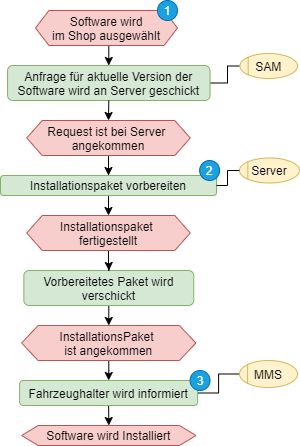
\includegraphics[width=0.8\columnwidth]{pictures/konzept-Eigene-Installation.png}
	\label{img:eigenstaendigIns}
	\caption{Eigenständige Installation von Software}
\end{figure}
\subsubsection{Kommunikationsprotokoll: Installationsvorschlag von Service Provider}
Abbildung \hyperref[img:installationsProtokollExtern]{11} stellt den Ablauf einer Service Registrierung dar. Stellen Sie sich folgende Situation vor: Sie sitzen in ihrem Fahrzeug und möchten in die Innenstadt. Das Fahrzeug schlägt ihnen vor einen Parkplatz nahe der Fußgängerzone anzusteuern. Das Fahrzeug fährt dort hin ohne zu wissen, dass für die Nutzung des Parkplatzes eine Software notwendig ist, welche die Kommunikation mit dem Parkautomaten ermöglicht. Das Protokoll setzt ein, sobald das Fahrzeug am Parkplatz ankommt. Es fährt in eine Zone die vom Parkautomaten überwacht wird \textit{(1)}. Wird ein Fahrzeug erkannt, versucht der Parkautomat sich beim Fahrzeug zu registrieren. Ist die Nachricht im Fahrzeug angekommen wird überprüft, ob bereits eine Software auf dem Fahrzeug installiert ist welche die Nachrichten verarbeiten kann \textit{(2)}. Dies wird anhand der Software ID gemacht.\\
Ist die Software bereits installiert, wird überprüft ob die installierte Version der Software aktuell ist. Wenn ja, kann der Service genutzt werden. Dieser Ablauf wird im kommenden Kapitel vorgestellt. Ist die Software noch nicht Installiert oder die installierte Version ist nicht mehr aktuell wird der Fahrzeughalter gefragt, ob er die Software Aktualisieren bzw. Kaufen möchte \textit{(4)}. Dies geschieht über eine Eingabe in der Mensch-Maschine-Schnittstelle. Wird diese Anfrage abgelehnt, wird keine Software installiert und das Fahrzeug verlässt die Registrierungszone wieder. Andernfalls sendet das Fahrzeug eine Installationsanfrage an den Server, welche das Manifest des Fahrzeugs und Informationen zur Software beinhaltet. Der Server nimmt die Anfrage an und erstellt ein Installationspaket für die entsprechende Software \textit{(5)}. Ist das Paket fertig, wird es an das Fahrzeug verschickt. Handelt es sich um ein Update einer bereits installierten Software, trifft der Fahrer keine Kaufentscheidung sondern akzeptiert die neuen Bedingungen der Software. Haben sich diese nicht geändert, wird das update automatisch durchgeführt. Muss die Software neu gekauft werden, trifft der Fahrzeughalter ein Kaufentscheidung. Er kann das ihm vorgestellte Angebot entsprechend seiner Bedürfnisse für die Software anpassen \textit{(Leihe statt Kauf, etc.)}.
\begin{figure}[!h]
	\centering
	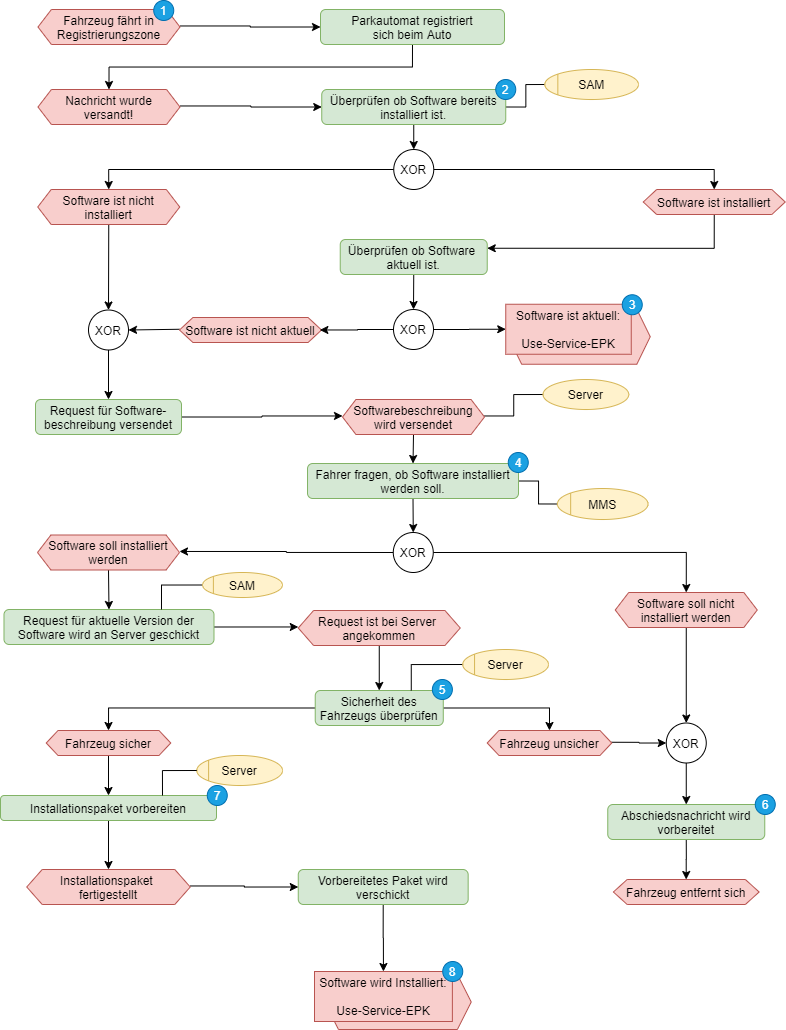
\includegraphics[width=0.86\columnwidth]{pictures/konzept-Installationsprozess.png}
	\label{img:installationsProtokollExtern}
	\caption{Installationsprozess von Software}
\end{figure}
\subsubsection{Kommunikationsprotokoll: Nutzung eines Service}
Das letzte Kommunikationsprotokoll wird genutzt, wenn ein Service vom Fahrzeughalter genutzt wird. Dies passiert \textbf{immer} direkt nach dem vorherigen Kommunikationsprotokoll, wenn die installierte Software aktuell ist \textit{(1)}. Der Service wird dem Fahrzeughalter über die Mensch-Maschine-Schnittstelle angezeigt \textit{(2)} und der Fahrer muss entscheiden, ob er diesen nutzen möchte oder nicht. Die Antwort wird an den Parkautomaten gesendet \textit{(3)}, welcher die Entscheidung des Fahrers auswertet. Wurde der Service abgelehnt, wird eine Abschiedsnachricht zusammen mit einer Aufforderung das Gelände zu verlassen an das Fahrzeug gesendet. Wurde der Service angenommen, beinhaltet die zurückgeschickte Nachricht einen zugewiesenen Parkplatz und ein Parkticket. Das Fahrzeug verarbeitet die Nachricht\textit{(4)}, zeigt diese auf der Mensch-Maschine-Schnittstelle an und steuert den Wagen entsprechend der Nachricht.
\begin{figure}[!h]
	\centering
	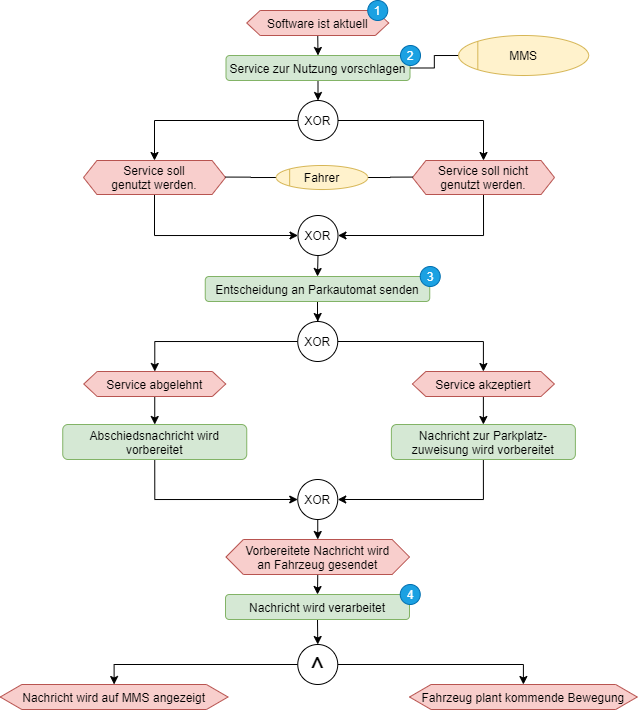
\includegraphics[width=0.75\columnwidth]{pictures/konzept-Nutzungsprozess.png}
	%	\label{}
	\caption{Nutzungsprozess von Software}
\end{figure}
\clearpage
\subsection{Ausblick}
Die in diesem Kapitel erstellten Konzepte wurden mit der Intention entwickelt, einzelne Bausteine der Wertschöpfungskette zu unterstützen. In Kapitel \ref{wsk} wurden weitere Konzepte und notwendige Arbeitsvorgänge vorgeschlagen, für welche ebenfalls technische oder zumindest theoretische Konzepte zu erstellen sind.\\
Im Hinblick auf den Prototypen wurden Kommunikationsprotokolle erstellt, welche für die Einbindung in eine Uptane-basierte Fahrzeug-Server-Kommunikation anwendbar sind. Der Ablauf der Protokolle, die im Forschungsseminar erarbeitete Softwarearchitektur und auch weitere in der Arbeit gewonnene Erkenntnisse und Ideen werden im folgend vorgestellten Prototypen visuell veranschaulicht werden.\\
\\
\\
\\
\\
\\
\\
\\
\\
\\
\\